\chapter{Introduction}\label{ch:introduction}

% The scope of the work includes software and analysis.

The scope of this work includes development and validation of \Cyder, a generic 
repository software library for modeling various long-term disposal system concepts 
for nuclear material. \Cyder is integrated with the \Cyclus 
computational fuel cycle systems analysis platform in order to inform 
repository performance metrics with respect to candidate fuel cycle options.  
By abstraction of more detailed models, this work captures the dominant physics 
of radionuclide and heat transport phenomena affecting repository performance 
in various geologic media and as a function of arbitrary spent fuel 
composition. 

\section{Motivation} 
% Provide a brief description of the importance of the work (what problem it 
%   addresses/solves):

The development of sustainable nuclear fuel cycles is a key challenge as the 
use of nuclear power expands domestically and internationally.  Accordingly, 
the United States and other nations are considering a number of nuclear fuel 
cycle and geologic disposal options simultaneously \cite{doe_strategy_2013, 
von_lensa_red-impact_2008}.  These decisions 
are technologically coupled by repository capacity. That is, 
radionuclide containment performance of a geologic repository is, in part, a function of 
spent fuel and high level waste composition, which varies among fuel cycle 
options. For this reason, integration of a generic disposal model and a fuel 
cycle systems analysis framework is necessary to illuminate performance 
distinctions of candidate repository host media, designs, and engineering 
components in the context of fuel cycle options.  In answer to this need, \Cyder 
integrates with the \Cyclus computational fuel cycle systems analysis platform 
\cite{huff_cyder_2013,wilson_cyclus:_2012}. 


% The approach must also be modular to support combinatorially complex 
% decision space 

To support analysis of numerous combinatoric fuel cycle possibilities, a 
top-level simulation tool capable of modular substitution of various fuel cycle 
facility, repository, and engineered barrier components is needed. The modular 
natural and engineered barrier representations resulting from this work will assist in 
informing current technology choices, identifying important parameters 
contributing to key waste disposal metrics, and highlighting the most promising 
waste disposal combinations with respect to metrics chosen by the user. 

% Speed

System level fuel cycle simulation tools must facilitate efficient sensitivity 
and uncertainty analyses and simulation of a wide range of fuel cycle 
alternatives. Therefore, a generic repository model appropriate for systems 
analysis must emphasize speed in accordance with use cases requiring repeated 
simulations. Simultaneously, it must provide modeling options at a level of 
detail that successfully captures significant aspects of the underlying 
physics.  Often termed abstraction, the process of simplifying while 
maintaining the salient features of the underlying physics is the method by 
which thermal and radionuclide transport models were developed in this work. 

% The fuel cycle parameters that may be varied are numerous and coupled to the 
% back end.

Fuel cycle parameters of particular interest in fuel cycle systems 
analysis have historically been those related to the front end of the fuel 
cycle.
However, parameters representing decisions concerning the back end
of the fuel cycle are of increasing interest as the United States further
investigates repository alternatives to Yucca Mountain.  Parameters such as
repository geology, engineered barriers, appropriate loading strategies and
schedules are all independent parameters up for debate. Due to the feedback 
implication of repository capacity and performance, these
parameters are coupled with decisions about the fuel cycle. 

% So we need a full systems analysis package, incorporating a repository. 

Thus, coupled parameters require full synthesis with a systems analysis code 
that dynamically and appropriately determines the isotopic mass flows into the 
repository, their appropriate conditioning, densities, and other physical 
properties.  

\subsection{Future Fuel Cycle Options}

% DOE is interested in many fuel cycle options. 
% DOE is considering 3 main options, each of which pose different waste 
% management challenges . . .

As the United States and other nations seek to develop technologies and strategies to support a 
sustainable future for nuclear energy, various fuel cycle strategies and 
corresponding disposal system options are being considered.  Specifically, the 
domestic fuel cycle option space under current consideration is described in 
terms of three distinct fuel cycle categories with the monikers Once Through, 
Full Recycle, and Modified Open. Each category presents unique disposal system 
design challenges. Systems analyses for evaluating these options must 
be undertaken in order to inform a national decision to deploy a comprehensive 
fuel cycle system by 2050 \cite{doe_nuclear_2010}. 

% Once through presents capacity issues . . . 

The Once-Through Cycle category includes fuel cycles similar to the fuel cycle 
currently deployed in the United States, utilizing light water reactors and 
direct disposal of spent nuclear fuel in a geologic repository.
Such fuel cycles neglect reprocessing and present challenges associated with 
high volumes of minimally treated spent fuel streams.  In in a geologic 
repository a business as usual 
scenario, conventional power reactors comprise the majority of nuclear energy 
production. 
Calculations from the Electric Power Research Institute corroborated by 
the \gls{US} \gls{DOE} in 2008 indicate that without an increase in the statutory 
capacity limit of the \gls{YMR}, continuation of the current Once Through fuel 
cycle will generate a volume of spent fuel that will necessitate
the siting of an additional federal geologic repository to accommodate spent 
fuel \cite{kessler_room_2006, doe_report_2008}. 

% Full Recycle presents the issue of variable waste streams. . .

A Full Recycle option, on the other hand, requires the research, development, 
and deployment of partitioning, transmutation, and advanced reactor technology 
for the reprocessing of used nuclear fuel.  In this scheme, conventional 
once-through reactors will be phased out in favor of advanced transmutation 
technologies. All fuel in the Full Recycle strategy will be 
reprocessed using an accelerator driven system or by 
cycling through an advanced fast reactor. Such fuel may undergo partitioning, 
the losses from which will require waste treatment and ultimate disposal in a 
repository. Thus, a repository under the Full Recycle scenario must support
a waste stream composition that is highly variable during transition periods as 
well as myriad waste forms and packaging associated with isolation of differing 
waste streams.

% Modified Open presents both problems. . . 

Finally, the Modified Open Cycle category of options includes a variety of fuel 
cycle options that fall between once through and fully closed. Advanced fuel 
cycles such as deep burn and small modular reactors will be considered as will 
partial recycle options.  Partitioning and reprocessing strategies, however, 
will be limited to simplified chemical separations and volatilization. This 
scheme presents a dual challenge in which spent fuel volumes 
and composition will both vary dramatically among various possibilities within 
this scheme \cite{doe_nuclear_2010} .

% Various waste streams require various WFs and WPs 

Clearly, the waste streams resulting from potential fuel cycles present an 
array of corresponding waste disposition, packaging, and engineered barrier 
system options. Differing spent fuel composition, partitioning, transmutation, 
and chemical processing decisions upstream in the fuel cycle may demand differing 
natural and engineered barrier requirements during disposal. The 
capability to model thermal and radionuclide transport phenomena of 
arbitrary isotopic compositions is therefore required. This work has produced a 
disposal system simulator that meets this need. 


\subsection{Future Waste Disposal System Options}

% DOE is thinking about various geologies

In addition to reconsideration of the domestic fuel cycle policy, the uncertain 
future of the \gls{YMR} has driven the expansion of the option space of 
potential repository host geologies to include, at the very least, granite, 
clay/shale, salt, and deep borehole concepts \cite{nutt_used_2010}. 

% Various waste forms, packages, etc. are being considered.

In accordance with various fuel cycle options, corresponding waste form, waste 
package, and other engineered barrier systems are being considered.  
Specifically, current considerations include ceramic (e.g.  Uranium Oxide), 
glass (e.g.  borosilicate glasses), and metallic (e.g.  hydride fuels) waste 
forms. Waste packages may be copper, steel, or other alloys. Similarly, buffer 
and backfill materials vary from the crushed salt recommended for a salt 
repository to bentonite or concrete in other geologies. Therefore, this repository  
model was designed to be capable of modular substitution of waste form models and data
in order to analyze the full option space.

% Various geologies, WFs, WPs, EBSs have various physics

The physical, hydrologic, and geochemical mechanisms that dictate 
radionuclide and heat transport vary between the geological and engineered 
containment systems in the domestic disposal system option space.  Therefore, 
to support the system level simulation effort, a disposal system model must
capture the salient physics of these geological options and quantify associated 
disposal metrics.  Furthermore, in the same way that system level 
modularity facilitates analysis, so too does modular linkage between subcomponent 
process modules. The subcomponent models and repository environmental model in 
this work therefore provide a cohesively integrated disposal system simulator.


\subsubsection{Thermal Modeling Needs}
% repository loading limits
% optimization of layout
% necessary decay cooling time before emplacement.
The decay heat from nuclear material generates a significant heat source within a 
repository. In order to arrive at loading strategies that comply with thermal 
limits in the engineered barrier system and the geological medium, a thermal 
modeling capability has been included in the repository model. 


Partitioning and transmutation of heat generating radionuclides within  some 
fuel cycles will alter the heat evolution of the repository 
\cite{swift_applying_2010}. Thus, to distinguish  between the repository heat 
evolution associated with various fuel cycles involving partitioning and 
transmutation, the repository analysis model must, at the very least, capture 
the decay heat behavior of dominant heat contributors.  Isotopes of plutonium, 
americium, and their decay daughters dominate decay heat contribution within 
used nuclear fuels. Other high heat contributing radionuclides include isotopes 
of cesium, strontium, and curium \cite{piet_which_2007}. 

Thermal limits and heat evolution within a used nuclear fuel disposal system are engineered 
barrier and geology dependent. 
The size, design, and loading strategy of the waste form, package, and tunnel 
loading strategies are constrained by both technical and legislative limits. 

Thermal limits of various \glspl{EBS} have their technical basis in the 
temperature dependence of isolation integrity of the waste form. Waste form 
alteration, corrosion, degradation, and dissolution behavior is a function of heat in 
addition to redox conditions and constrains loading
density within the waste form. 

Thermal limits of the geologic environment can be based on the mechanical 
integrity of the rock as well as mineralogical, hydrologic and geochemical 
phenomena. The isolating characteristics of a geological environment are most 
sensitive to hydrologic 
and geochemical effects of thermal loading. Thus, heat load constraints are 
typically chosen to control hydrologic and geochemical response to thermal 
loading. In the United States, current regulations necessitate thermal limits in 
order to passively steward the repository's hydrologic and geochemical integrity 
against radionuclide  release for the first 10,000 years of the repository.

Constraints for a broad set of possible geological environments 
depend on heat transport properties and geochemical behaviors of the rock matrix 
as well as its hydrologic state.  Such constraints affect the  
repository waste package spacing and repository footprint among 
other parameters. 

Since some 
material and hydrologic phenomena affecting radionuclide transport are 
thermally coupled, future advanced implementation goals include informing those 
parameters with the thermal modeling capability developed here. 

%Clay repositories should have a ~70 degrees C limit, because temps higher than 
%100 degrees can cause irreversible minerological damage.
%From ANDRA:
%``In order to remain in an operational range in which phenomena are known and, 
%thus, reduce any damage to the argillite, the objective is to restrict 
%argillite temperature to these values. Basically, it means that the thermal 
%dimensioning of the cells and the architecture of the C waste repository zone 
%aim to restrict the temperature to 90°C at the interface “disposal cell – 
%argillite” and to ensure that the temperature will be below 70°C, in the 
%geological medium on the cell boundary, before a thousand years, which provides 
%a safety margin with respect to thermal effects.''

In addition to development of a concept of heat transport within the repository 
in order to meet heat load limitations, it is also necessary to model 
temperature gradients in the repository in  order to support modeling of 
thermally dependent hydrologic and material phenomena.  As mentioned above, 
waste form corrosion processes, waste form
dissolution rates, diffusion coefficients, and the mechanical integrity of 
engineered barriers and geologic environment are coupled with temperature 
behavior. 
Only a coarse time resolution is necessary to capture that coupling 
however, since time evolution of repository heat is
such that thermal coupling can typically be treated as quasi static for long 
time scales.
\cite{andra_argile:_2005}. %andra, clay, evaluation, page 195)

\subsubsection{Source Term Modeling Needs}

Domestically, the \gls{EPA} has defined a limit on  human 
exposure due to the repository. This regulation places important limitations on 
capacity, design, and loading techniques for repository concepts under 
consideration. Repository concepts developed in this work must therefore 
quantify radionuclide transport through the geological environment in order to 
calculate repository capacity and other postprocessed performance metrics. 

The exposure limit set by the \gls{EPA} is based on a `reasonably maximally 
exposed individual.' For the \gls{YMR}, the limiting case is a person who lives, 
grows food, drinks water and breathes air 18 km downstream from the repository. 
The Yucca Mountain Repository \gls{EPA} regulations limit total dose from the 
repository to 15 mrem/yr, and limit dose from drinking water to 4 mrem/yr for 
the first 10,000 years. 
Predictions of that dose rate depend on an enormous variety of factors, most 
important of which is the primary pathway for release. In the \gls{YMR} primary 
pathway of radionuclides from an accidental release will be from cracking aged 
canisters. Subsequently, transport of the radionuclides to the water table 
requires that the radionuclides come in contact with water and travel through 
the rock to the water table. This results in contamination of drinking water 
downstream.  

Source term is a measure of the quantity of a radionuclide released into the 
environment whereas radiotoxicity is a measure of the hazardous effect of that 
particular radionuclide upon human ingestion or inhalation.  In particular, 
radiotoxicity is measured in terms of the volume of water dilution required to 
make it safe to ingest. Studies of source term and radiotoxicity therefore make 
probabilistic assessments of radionuclide release, transport, and human 
exposure.  

Importantly, due to the long time scale and intrinsic uncertainties required in 
such probabilistic assessments it is in general not advisable to base any 
maximum repository capacity estimates on source term. This is due to the fact 
that in order to give informative values for the risk associated with transport of 
particular radionuclides, for example, it is necessary to make highly uncertain  
predictions concerning waste form degradation, water flow, and other parameters 
during the long repository evolution time scale.  However, source term remains a 
pertinent metric for the comparison of alternative separations and fuel cycle
scenarios as it is a fundamental factor in the calculation of risk.
%The probabilistic nature of these assessments mean a direct dependence of 
%source term on repository capacity can be difficult to arrive at.  

Arriving at a generalized metric of probabilistic risk is fairly difficult. For 
example, the \gls{PEI} metric from Berkeley (ref.  
\cite{bouvier_comparison_2007}) is a multifaceted function of spent fuel 
composition, waste conditioning, vitrification method, and radionuclide 
transport through the repository walls and rock.  Also, it makes the assumption 
that the waste canisters have been breached at $t=0$. Furthermore, reported in 
$m^3$, PEI is a measure of radiotoxicity in the environment in the event of 
total breach. While informative, this model on its own does not completely 
determine a source-term limited maximum repository capacity.  Additional waste 
package failure and a dose pathway model must be incorporated into it.


\subsection{Domestic Research and Development Program}

The DOE-NE Fuel Cycle Technology (FCT) program has three groups of relevance to 
this effort: these are the \gls{UFD}, the \gls{SWF}, and \gls{FCO} (previously 
Systems Analysis) campaigns.  
The \gls{UFD} campaign is conducting the \gls{RDD} related to the storage, 
transportation, and disposal of radioactive wastes generated under both the 
current and potential advanced fuel cycles.  The SWF campaign is conducting 
\gls{RDD} on potential waste forms that could be used to effectively isolate 
the 
wastes that would be generated in advanced fuel cycles.  The \gls{SWF} and
\gls{UFD} campaigns are developing the fundamental tools and information base 
regarding the performance of waste forms and geologic disposal systems.  The 
\gls{FCO} campaign is developing the overall fuel cycle simulation tools and 
interfaces with the other FCT campaigns, including \gls{UFD}.  

This effort has interfaced with those campaigns to develop the higher level
dominant physics representations for use in fuel cycle system analysis tools.
Specifically, this work has leveraged conceptual framework development and
primary data collection underway within the Used Fuel Disposition Campaign. 

It has also benefited from University-laboratory collaboration via work by 
Radel, Wilson, Bauer et. al. to model repository behavior as a function of the 
contents of the waste \cite{radel_effect_2007}.  




\section{Methodology} 
% Overview : 
% put a repository model into cyclus
% that is capable of distinguishing between disposal choices
% and fuel cycle choices
% but is still speedy. 

\begin{frame}[ctb!]
  \frametitle{Methodology : Modularity }
  A modular repository framework facilitates 
  \begin{itemize}
    \item  interchangable subcomponents (e.g. buffer material) so that 
      the impact on the disposal system performance may be observed
    \item and simulations with varying levels of detail.
  \end{itemize}
 \pause
  Integration with a fuel cycle simulator facilitates
  \begin{itemize}
    \item analysis of feedback effects upon the fuel cycle
    \item and investigation of fuel cycle choices on disposal system 
      performance.
  \end{itemize}
\end{frame}

\begin{frame}[ctb!]
  \frametitle{Methodology : Abstraction for Efficiency}

  \begin{minipage}{0.49\textwidth}
      Abstraction simplifies models while capturing salient physics. 
      Parametric analysis with detailed models will inform simpler models at the 
      level of detail important for fuel cycle analysis.
    \begin{figure}[h!]
        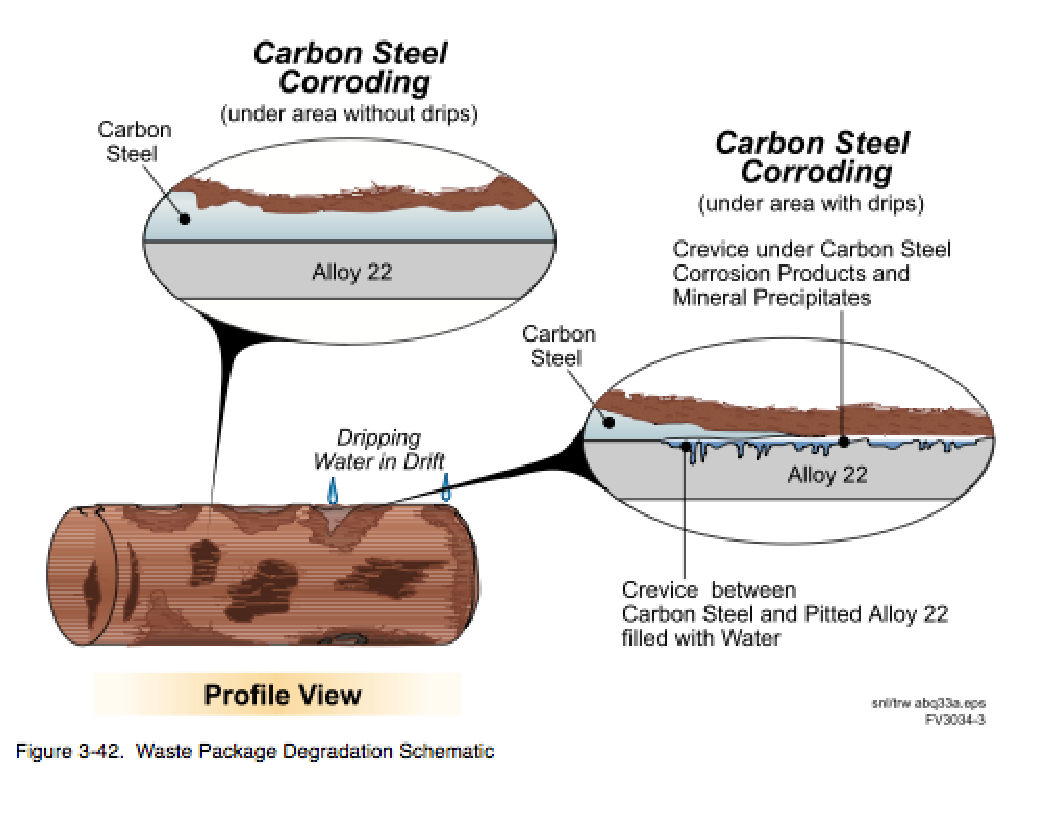
\includegraphics[width=\textwidth]{./images/reality.eps}
      \caption{A complex computational model is an abstraction of reality 
      \cite{doe_viability_1998}.}
      \label{fig:reality}
    \end{figure}
  \end{minipage}
  \hspace{0.01cm}
  \begin{minipage}{0.49\textwidth}
    \begin{figure}[h!]
        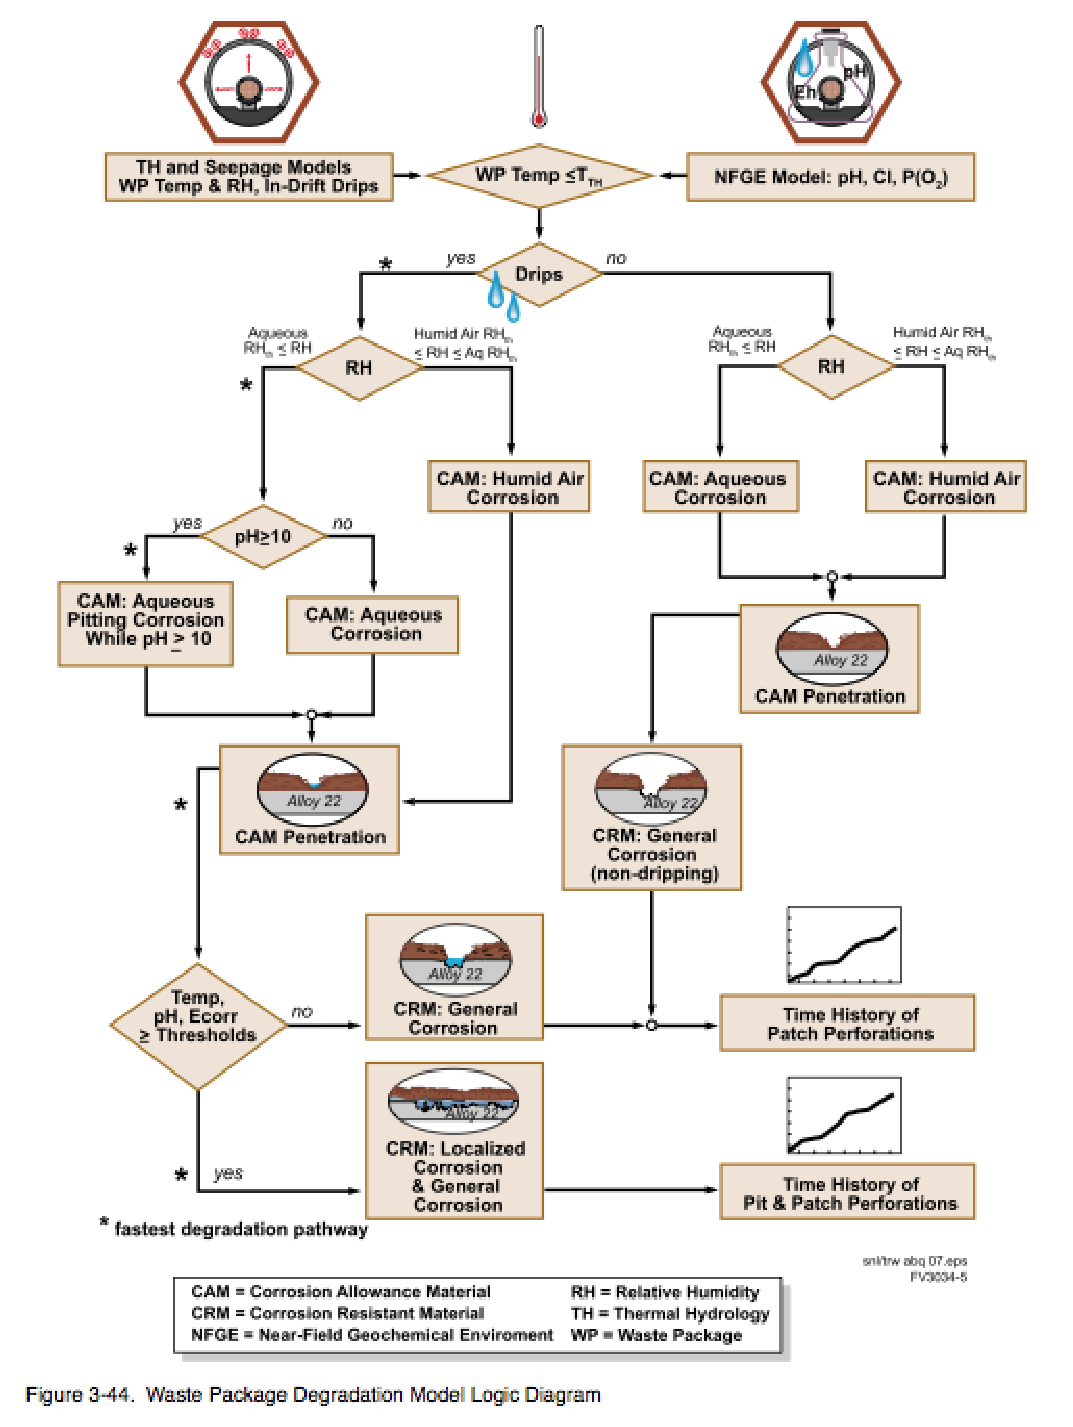
\includegraphics[width=0.9\textwidth]{./images/model.eps}
    \end{figure}
  \end{minipage}
  

\end{frame}


\section{Research Goals}

The purpose of this work was to design a fast, flexible code for medium
fidelity analysis of generic repository performance in the context of fuel
cycle analysis. In addition to implementing fundamental modeling capabilities,
\Cyder has been designed to provide an accommodating foundation for the
development of advanced capabilities in the future.

Cyder has implemented the following modeling capabilities :

\begin{itemize}
  \item Repository Concept Generality
    \begin{itemize}
      \item generic spatial loading
      \item modular component arrangement
      \item encapsulation of models and data
    \end{itemize}
  \item Radionuclide Transport Modeling 
    \begin{itemize}
      \item varying levels of detail
      \item component level detail
      \item solubility limitation and sorption modeling
      \item waste form degradation
      \item waste package failure
    \end{itemize}
  \item Thermal Modeling
    \begin{itemize}
      \item capturing the effect of spacing
      \item capturing the effect of differing media
    \end{itemize}
  \item Dynamic Fuel Cycle Simulation Feedback
\end{itemize}

Cyder was also designed to be used and developed by a community of people. \Cyder possesses the following user and developer features
\begin{itemize}
  \item User Features
    \begin{itemize}
      \item modular to accommodate the inherently modular combinatoric repository design options
      \item fast to accommodate parameretrized runs
      \item integrated to inform the dynamic effects of repository capacity features
    \end{itemize}
  \item Developer Features
    \begin{itemize}
      \item Open Source Framework
      \item Testing Framework
      \item Component Modularity to allow future development and customization
    \end{itemize}
\end{itemize}

% Summarize document

A literature review, Chapter \ref{ch:litrev}, presents background material that organizes and 
reports upon previous relevant work. First it summarizes the state of the art of 
repository modeling integration within current systems analysis tools. It then 
describes current domestic and international disposal system option space. 
Next, the literature review focuses upon current analytical and 
computational modeling of radionuclide and heat transport through various waste 
forms, engineered barrier systems, and geologies of interest.  It also 
addresses previous efforts in generic geologic environment repository modeling in order to 
categorize and characterize detailed computational models of radionuclide and 
heat transport available for abstraction and validaton efforts.

% modeling paradigm

Chapter \ref{ch:paradigm} details the computational paradigm of the \Cyclus 
systems analysis platform and \Cyder repository model which constitute this work. 
It describes the \Cyclus fuel cycle simulation context which drives fundamental 
\Cyder design descisions as well as the modular paradigm emphasized in both 
\Cyclus and \Cyder. 

% methodology

Chapter \ref{ch:methodology} develops  radionuclide transport and heat transport 
models based on an abstraction process between analytic models and the results 
of detailed tools.  These models, representing engineered barrier and geological 
disposal system components, are defined by their interfaces and their 
relationships as interconnected modules, distinctly defined, but coupled.  This 
modular implementation allows exchange  of technological options for comparison 
as well as exchange of models for the same technological option with varying 
levels of detail.  

% Test Cases and Benchmarks

Chapter \ref{ch:demonstration} describes simulation cases conducted to 
demonstrate radionuclide transport and thermal capacity analysis capabilities in \Cyder. It 
also describes verification and validation procedures which benchmarked \Cyder 
behavior against analytic solutions and more detailed models.


% Conclusions
Finally, in Chapter \ref{ch:conclusions}, contributions to the field and 
suggested future work are summarized. 



%%%%%%%% %%%%%%%% %%%%%%%% %%%%%%%% %%%%%%%% %%%%%%%% %%%%%%%% %%%%%%%%
%%%%%%%% %%%%%%%% %%%% These chapters may be saved for the thesis . . .  
%%%%%%%% %%%%%%%% %%%%%%%% %%%%%%%% %%%%%%%% %%%%%%%% %%%%%%%% %%%%%%%% 

% Chapter \ref{ch:ebs} will adapt existing models and data to the development of 
% concise dominant physics waste form, waste package, and other engineered 
% barriers (i.e., bentonite or cementitious materials) models appropriate for 
% treatment of key radionuclides within the waste streams.  Material/barrier 
% degradation, radionuclide release, and radionuclide transport, and thermal 
% processes and effects will be included, as necessary, in the concise 
% representations that will be developed for subsequent use in the system-level 
% architecture. A range of waste forms, waste package materials, and other 
% engineered barrier materials (buffer, backfill) under consideration by the 
% DOE-NE FCT program (SWF and UFD campaigns) will be evaluated. The concise 
% dominant physics models will include appropriate load limiting factors of the 
% stabilizing medium and waste packaging including such as waste composition, 
% chemical form, and heat generation.
% 
% Chapter \ref{ch:extension} will discuss the future work necessary to extend 
% developed models to comprehensively cover the potential disposal system option 
% space. The path forward for extension of the geological base case model to 
% cover all five geologic concepts of interest (clay/shale, granite, salt, and 
% deep boreholes) will be discussed. Similarly, gaps in waste form and 
% engineered barrier system models and data will be addressed and a plan for 
% data and model coverage for that options space will be described.

